\chapter{Artefact Design} \label{chap:artefact-design}
\section{Development decisions}
\subsection{Software development methodology}
In the software development life cycle there are various stages: requirements gathering, analysis, design,
development, testing, deployment and maintenance.\\
The Agile software development methodology will be utilised in this project; and this project will be separated
into various iterations of design, development, and testing. This will allow for a more flexible approach to
the task and the ability to make changes as the project progresses without requiring additional time and effort
to fully test and deploy an inaccurate or unsuitable artefact.
\begin{figure}
    \centering
    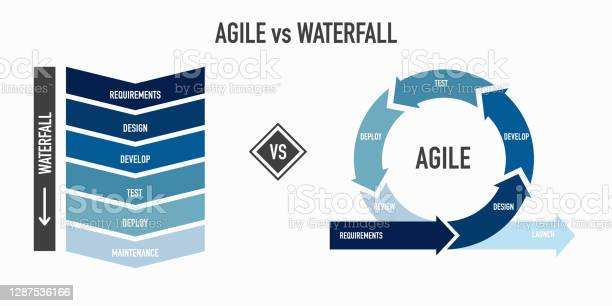
\includegraphics[width=\columnwidth]{figures/development_methodologies.jpg}
    \caption{A comparison of the Agile and Waterfall methodologies (source: iStock, iam2mai)
    (replace as there is a copyright)}
    \label{fig:development_methodologies}
\end{figure}
\FloatBarrier

\subsection{Software languages and libraries}
\subsubsection{Programming Language}
Python has been chosen to be used in this project as it is ubiquitous for artificial intelligence related
tasks. There are many resources readily available for Python with regards to its usage on artificial
intelligence models and neural networks. There are various Python libraries for machine learning applications
such as Tensorflow, an `end-to-end open source machine learning platform' created by Google as well as
PyTorch, ` open source machine learning framework' created by Facebook's AI Research Lab.

\subsubsection{Python libraries for machine learning}
As mentioned in the previous section there are various machine learning libraries for Python. Currently, the
most popular is Tensorflow and has the most resources available.
However, the usage of PyTorch has accelerated over the past years and is quickly becoming the preferred
library as it is considered to be more `pythonic' and often quicker to train neural networks.

Tensorflow will be used in the project due to its current ubiquity in this task, especially surrounding
its applications for financial forecasting. However, PyTorch may be chosen for future iterations if
the performance of Tensorflow is found to be insufficient and the performance of PyTorch is found to be
greater.

\section{Input features chosen and data collection}
The input features chosen are an amalgamation primarily based on those found in the literature review.
From the literature review, the input features have been classified into four categories:
\begin{itemize}
    \item Stock market index
    \item Money availability
    \item Alternative portfolio allocations
    \item Sentiment
\end{itemize}

From this, the following sources for input features have been chosen; the reasoning are explained and the
sources for used in the data collection process are also present within this list.
\begin{itemize}
    \item Stock market index
    \begin{itemize}
        \item Closing price\\
        \textbf{Reasoning:} It is believed that a sequence of closing price returns
        can be utilised to predict a future closing price\\
        \textbf{Source:} Yahoo Finance - SPY Historical Data:\\
        https://uk.finance.yahoo.com/quote/SPY/history
        \item Volume\\
        \textbf{Reasoning:} It is believed that the amount of stock traded can indicate
        confidence in that stock market index and potentially future price movements\\
        \textbf{Source:} Yahoo Finance - SPY Historical Data:\\
        https://uk.finance.yahoo.com/quote/SPY/history
        \item Volatility (based on VIX)\\
        \textbf{Reasoning:} It is believed that the volatility in the stock market can potentially
        indicate future price movements\\
        \textbf{Source:} Yahoo Finance - VIX Historical Data:\\
        https://uk.finance.yahoo.com/quote/\%5EVIX/history
    \end{itemize}
    \item Money availability
    \begin{itemize}
        \item M1 Money Supply\\
        \textbf{Reasoning:} It is believed that a change in total money supply circulation can affect
        the amount of money allocated to the stock market, such as with measures related to quantitative
        easing to affect stock returns\\
        \textbf{Source:} Federal Reserve Economic Data - M1 Money Supply:\\
        https://fred.stlouisfed.org/series/WM1NS
        \item GDP\\
        \textbf{Reasoning:} It is believed that the GDP can affect the money available to market
        participants and thus impact stock returns\\
        \textbf{Source:} Federal Reserve Economic Data - GDP:\\
        https://fred.stlouisfed.org/series/GDP
    \end{itemize}
    \item Alternative portfolio allocations
    \begin{itemize}
        \item Treasury Yields
        \begin{itemize}
            \item 1Mo
            \item 3Mo
            \item 1Yr
            \item 2Yr
            \item 5Yr
            \item 10Yr
            \item 20Yr
            \item 30Yr
        \end{itemize}
        \textbf{Reasoning:} It is believed that the market participants often allocate their funds
        to treasury bonds / bills / notes for a guaranteed return compared to risk in the stock market.
        A change to yields may affect the money allocated in the stock market and thus affect the
        return of the stock market index.\\
        \textbf{Source:} US Dept. of the Treasury - Treasury Par Yield Curve Rates:\\
        % \seqsplit{https://home.treasury.gov/resource-center/data-chart-center/interest-rates/TextView?type=daily_treasury_yield_curve}
        \item Effective Federal Funds Rate\\
        \textbf{Reasoning:} EFFR is the interest rate banks charge one another for overnight loans, a change in 
        EFFR may affect the loans banks make / take and thus affect the money the banks have available to allocate
        in the stock market; this may affect the return of the stock market index.\\
        \textbf{Source:} Federal Reserve Economic Data - EFFR:\\
        https://fred.stlouisfed.org/series/EFFR
        \item Repurchase / Reverse Repurchase Agreements\\
        \textbf{Reasoning:} A change in utilisation of repurchase agreements may indicate if banks expect
        a greater return elsewhere and how banks are allocating money. This may have an impact on the 
        return of the stock market index\\
        \textbf{Source:} New York Fed - Repo:\\
        https://www.newyorkfed.org/markets/desk-operations/repo
        \item Gold\\
        \textbf{Reasoning:} It is believed that a change in the prices of commodities such as gold may be
        an indicator of portfolio allocation changes; thus affecting the return of the stock market index\\
        \textbf{Source:} London Bullion Market Association - Precious Metal Prices:\\
        https://www.lbma.org.uk/prices-and-data/precious-metal-prices\#/table
        \item Foreign Currency
        \begin{itemize}
            \item USD-GBP\\
            \textbf{Source:} Federal Reserve Economic Data - GBP:\\
            https://fred.stlouisfed.org/series/DEXUSUK
            \item USD-EUR\\
            \textbf{Source:} Federal Reserve Economic Data - EUR:\\
            https://fred.stlouisfed.org/series/DEXUSEU
            \item USD-JPY\\
            \textbf{Source:} Federal Reserve Economic Data - GBP:\\
            https://fred.stlouisfed.org/series/DEXJPUS
        \end{itemize}
        \textbf{Reasoning:} It is believed that the currency exchange rates may be an indicator of confidence
        of the country of the currency, thus a change in currency rate may result in a change of portfolio
        allocations of participants in that country's stock market.        
    \end{itemize}
    \item Sentiment
    \begin{itemize}
        \item Put-to-Call Ratio\\
        \textbf{Reasoning:} It is believed that the market participants may use the options market
        to speculate on future returns of the stock market. The put to call ratio indicates the sentiment
        of the market participants and may have an affect on the return of the stock market index.\\
        \textbf{Source:} AlphaAlerts: Historical Equity Put/Call Ratio\\
        https://www.alphalerts.com/live-historical-equity-pcr/
        \item Employment Rate\\
        \textbf{Reasoning:} It is believed that market participants may react to changes of employment
        rate in making investment decisions. A change in nationwide employment may cause market participants
        to change their portfolio allocations due to lesser confidence in ability for companies in the country
        to produce and sell; thus potentially affect the return of the stock market index.\\
        \textbf{Source:} Federal Reserve Economic Data - Employment Rate:\\
        https://fred.stlouisfed.org/series/LREM64TTUSM156S
        \item Inflation Rate\\
        \textbf{Reasoning:} It is believed that a change in inflation rate can cause market participants
        to change their portfolio allocations and thus affect the return of the stock market\\
        \textbf{Source:} US Bureau of Labor Statistics - Inflation:\\
        https://www.bls.gov/data/\#prices
        \item Consumer Sentiment\\
        \textbf{Reasoning:} It is believed that a change in consumer sentiment towards the economy
        can cause market participants to change their portfolio allocations and thus affect the
        return of the stock market\\
        \textbf{Source:} University of Michigan - Consumer Sentiment:\\
        https://fred.stlouisfed.org/series/UMCSENT
        \item Consumer Confidence\\
        \textbf{Reasoning:} It is believed that a change in consumer confidence towards the economy
        can cause market participantsto change their portfolio allocations and thus affect the return
        of the stock market\\
        \textbf{Source:} Federal Reserve Economic Data - OECD Indicator for the US:\\
        https://fred.stlouisfed.org/series/CSCICP03USM665S
    \end{itemize}
\end{itemize}


\section{Assumptions made}
The primary assumptions are surrounding the trading days; whilst this varies per month / year, it is assumed
that 1 week is equivalent to 5 trading days, 1 month is equivalent to 21 trading days, 1 quarter (3 months)
is equivalent to 63 trading days, 1 half is equivalent to 126 trading days, and 1 year is equivalent to 252
trading days. These assumptions are made based on the NYSE trading hours that shows a month may have
between 19 to 23 trading days, each quarter may have 61 to 64 trading days, generally resulting in a total
of 252 trading days \parencite{nyse_2020}.

\section{Data preprocessing}
\subsection{Data normalisation}
For each input feature, the percentage change over the previous period is calculated. For example if the feature
is reported daily, the percentage change since the last day is calculated. For the closing price of the stock
market index, the percentage change since the last two days, last week, last month and last quarter were also
included.

\begin{table}[h]
    \centering
    \begin{tabular}{|c|c|}
        \hline
        Input Feature & Function Applied \\
        \hline\hline
        SPY Closing Price & \makecell{\% Change vs Previous Day \\
        \% Change vs Previous 2 Days\\
        \% Change vs Previous Week\\
        \% Change vs Previous Month\\
        \% Change vs Previous Quarter} \\
        SPY Volume & \% Change vs Previous Day \\
        VIX (Volatility Index) & \% Change vs Previous Day \\
        M1 Money Supply & \% Change vs Previous Week \\
        GDP & \% Change vs Previous Quarter \\
        \makecell{Treasury Yields\\
        (1 Month, 3 Months, 1 Year, 2 Years, 5 Years\\
        10 Years, 20 Years, 30 Years)}& \% Change vs Previous Day \\
        EFFR & \% Change vs Previous Day \\
        Repurchase Agreements & \% Change vs Previous Day \\
        Repurchase Agreements Rates & \% Change vs Previous Day \\
        Reverse Repurchase Agreements & \% Change vs Previous Day \\
        Reverse Repurchase Agreements Rates & \% Change vs Previous Day \\
        Gold Price & \% Change vs Previous Day \\
        GBP Exchange Rate & \% Change vs Previous Day \\
        EUR Exchange Rate & \% Change vs Previous Day \\
        JPY Exchange Rate & \% Change vs Previous Day \\
        Put-to-Call Ratio & \% Change vs Previous Day \\
        Employment Rate & \% Change vs Previous Month \\
        Inflation Rate & \% Change vs Previous Month \\
        Consumer Sentiment & \% Change vs Previous Month \\
        Consumer Confidence & \% Change vs Previous Month \\
        \hline
    \end{tabular}
    \caption{Table showing input features for Iteration 1}
    \label{tab:artefact_data_normalisation}
\end{table}
\FloatBarrier

Following this, the inputs are assumed to be normally distributed, and are scaled using the scale function of
scikit-learn's preprocessing library. Based on values of that input feature, they are scaled with the following
equation (\autoref{eq:sklearn-scale}):

\begin{equation}
    z = \frac{x - u}{s}
    \label{eq:sklearn-scale}
\end{equation}

where x is the sampled value, u is the mean of all of the samples, and s is the standard deviation of the samples.

This results in a value known as the z-score, a measure of how many standard deviations a value is from the mean value.
99.7\% of z-score should be between -3 and +3, but there may be outliers that exceed these values. In order to account for this,
all values are clipped to be within the range -3 and +3, and then this range is scaled to be between -1 and +1 for optimised
operation within the artificial intelligence models.

\subsection{Training / Validation Split}
The dataset includes data from November 2006 to March 2022; the dataset is split 80:20 between training data and
validation data. This means March 2019 is the cut off period betweeen the training and validation datasets. This
results in 2730 samples for the training data and 560 samples for the validation data after accounting for some
values that are removed due to them having N/A values.

\subsection{Data balancing}
In order to ensure the artificial intelligence models do not have any biases associated with them, each of the training
and validation datasets will be shuffled to ensure the model is able to generalise rather than learn. Furthermore, once
shuffled, the number of sequences that result in an positive trading day are counted as well as the number of sequences that result in
a negative day. The minimum of the two are chosen to ensure there is an even split of inputs that result in a positive trading day,
and inputs that result in a negative trading day.

\section{Iteration 1}
\subsection{Artificial intelligence model used}\label{ssec:iteration1_ai_model}
In the first iteration, the LSTM model was utilised in order to create the foundations for the CNN-LSTM model. The LSTM
consists of LSTM layers and Dense layers, with the final Dense layer having an output of 2, representing one output for
a negative day (0) and another for a positive day (1), and utilised the 'softmax' activation function to predict the
probabilities of each output. The LSTM and Dense layers utilised the 'tanh' (hyperbolic tangent) and 'relu'
(REctified Linear Unit) activation functions respectively.

The model was fit using the Adam optimiser with a learning rate of 0.001 and a decay of 1e-6. Adam is a popular
and efficient algorithms for gradient descent.
The "Sparse Categorical Crossentropy" loss function was utilised in the fitting of the model due to there being multiple
label classes. This calculates the loss as the negative sum of the differences between the true label and the log of the softmax
probability.

\subsection{Sequence length used}
A sequence length of 21 days (approximately 1 month) was used for each of the input features of this model.
This is a figure that has not in this iteration been tested to be the optimal sequence length, but with a short
test of various sequence lengths, it has been found to be sufficient to produce values over 50\% accuracy.
\subsection{Input features}
The input features for this model included all of the input features mentioned in \autoref{tab:artefact_data_normalisation}.

\subsection{Layers and layer sizes} \label{ssec:iteration1layers}
Various amounts of LSTM layers and Dense layers, as well as layer sizes for each were tested. The accuracy of each model varied
significantly. For each LSTM layer, there was also a:
\begin{itemize}
    \item Dropout layer of 0.4 meaning a set of neurons may be
    deactivated 40\% of the time at random; it is a method of regularisation to prevent overfitting.
    \item Batch normalisation layer meaning the outputs of that layer were scaled to aid efficiency of the model.
\end{itemize}
The following models were created and compared with the following variables:

\begin{table}[ht]
    \centering
    \begin{tabular}{|c|c|c|}
        \hline
        Layer Type & Number of Layers & Layer Size \\
        \hline\hline
        LSTM & 1, 2 & 32, 64 \\
        Dense & 2, 3 & 32, 64 \\
        \hline
    \end{tabular}
    \caption{Table showing layers and layer sizes for Iteration 1}
    \label{tab:iteration1_layers}
\end{table}
\FloatBarrier

\subsection{Diagram of model used}
The diagram below (\autoref{fig:iteration1_model}) shows the best model identified in iteration 1 of this project.
There are two LSTM layers with a layer size of 64; and two Dense layers, one with a layer size of 32 and one with
a layer size of 2. For the purposes of this diagram, the 'None' value of each layer's shape can be ignored.

From the diagram, it is shown that the input shape the first LSTM layer takes: (None, 21, 31); this represents the
fact there is a sequence length of 21 (trading days) and 31 input features.  This LSTM layer returns a sequence, so its
output has a shape of (None, 21, 64); it is fairly abstract but represents that there are 64 neurons in the next layer.
As the sequences are returned, the next layers also have input and output shapes of (None, 21, 64). The following LSTM
layer however does not return a sequence, so its output shape is (None, 64).
Dropouts and Batch Normalisation layers are added to aid with regularisation and optimisation of the model.
The next layer is a Dense layer, with an input shape of (None, 64) and an output of the shape (None, 32). An additional
dropout layer is applied here before transitioning to the final Dense layer that has an output shape of (None, 2)
which represents the fact there are two potential outputs for the inputs: whether the following day
is an positive or negative trading day.

\begin{figure}[ht]
    \centering
    \includegraphics[height=0.95\textheight]{figures/results/lstm/model.png}
    \caption[Diagram of iteration 1 layers]{Diagram of iteration 1 layers}
    \label{fig:iteration1_model}
\end{figure}
\FloatBarrier

\section{Iteration 2}
\subsection{Artificial intelligence model used}\label{ssec:iteration2_ai_model}
In the second iteration, the CNN model was utilised in order to create the foundations for the CNN-LSTM model. The CNN
consists of Conv1D layers and Dense layers, with the final Dense layer having an output of 2, representing one output for
a negative day (0) and another for a positive day (1), and utilised the 'softmax' activation function to predict the
probabilities of each output. The Conv1D and Dense layers utilised the 'relu' (REctified Linear Unit) activation
function.

The model was fit using the Adam optimiser with a learning rate of 0.001 and a decay of 1e-6. Adam is a popular
and efficient algorithms for gradient descent.
The "Sparse Categorical Crossentropy" loss function was utilised in the fitting of the model due to there being multiple
label classes. This calculates the loss as the negative sum of the differences between the true label and the log of the softmax
probability.

\subsection{Sequence length used}
Contrary to the LSTM model, the CNN model does not use a sequence of historic data; it only uses the previous day's
data as the input to the model.

\subsection{Input features}
The input features for this model included all of the input features mentioned in \autoref{tab:artefact_data_normalisation}.

\subsection{Layers and layer sizes} \label{ssec:iteration2layers}
Various amounts of Conv1D layers and Dense layers, as well as layer sizes for each were tested. The accuracy of each model varied
significantly. For each Conv1D layer, there was also a MaxPooling1D layer following it; this created a downsampled
feature map which aids in optimising the model's efficiency.

Following the Conv1D layers, there was also a Flatten layer applied to ensure the the following Dense layers
were able to accept the shape of the output of the Convolutional layers.

The following models were created and compared with the following variables:

\begin{table}[ht]
    \centering
    \begin{tabular}{|c|c|c|}
        \hline
        Layer Type & Number of Layers & Layer Size \\
        \hline\hline
        Conv1D & 1, 2 & 16, 32 \\
        Dense & 1, 2 & 32, 64 \\
        \hline
    \end{tabular}
    \caption{Table showing layers and layer sizes for Iteration 2}
    \label{tab:iteration2_layers}
\end{table}
\FloatBarrier

\subsection{Diagram of model used}
The diagram below (\autoref{fig:iteration2_model}) shows the best model identified in iteration 2 of this project.
There is one Conv1D layer with a layer size of 32; and one Dense layer with a layer size of 2.
For the purposes of this diagram, the 'None' value of each layer's shape can be ignored.

From the diagram, it is shown that the input shape the first Conv1D layer takes: (None, 1, 31); this represents the
fact there are 31 input features.  This Conv1D layer has an output shape of (None, 1, 32); it is fairly abstract
but represents that there are 32 neurons in the next layer. This output is then passed to the MaxPooling1D Layer
which downsamples it to create a feature map. A Flatten layer is applied to mutate the shape from (None, 1, 32) to 
(None, 32) beforetransitioning to the final Dense layer that has an output shape of (None, 2)
which represents the fact there are two potential outputs for the inputs: whether the following day
is an positive or negative trading day.

\begin{figure}[ht]
    \centering
    \includegraphics[width=0.95\columnwidth]{figures/results/cnn/model.png}
    \caption[Diagram of iteration 2 layers]{Diagram of iteration 2 layers}
    \label{fig:iteration2_model}
\end{figure}
\FloatBarrier